\documentclass[hidelinks,12pt]{article}

\usepackage[brazil]{babel}
\usepackage[utf8]{inputenc}
\usepackage{amsmath}
\usepackage{amsfonts}
\usepackage{amssymb}
\usepackage{indentfirst}
\usepackage{color}
\usepackage{mathrsfs}
\usepackage{pgfplots}
\usepackage{hyperref}
\usepackage{fancyhdr}
\usepackage{graphicx}
\usepackage[export]{adjustbox}
\newcommand{\icon}[1]{\includegraphics[height=12pt]{#1}}
\newcommand{\bigicon}[1]{\includegraphics[height=50pt]{#1}}

\newcommand{\iconb}[1]{\includegraphics[height=20pt]{#1}}
\setcounter{secnumdepth}{5}

\fancypagestyle{plain}{%
	\fancyfoot{}%
	\fancyhead{}%
}


\begin{document}
\pagenumbering{gobble}
\pagestyle{fancy}


\lhead{\bigicon{Figures/ufu}}
\chead{{\footnotesize UNIVERSIDADE FEDERAL DE UBERLÂNDIA \\ FACULDADE DE CIÊNCIA DA COMPUTAÇÃO \\ Inteligência Computacional} \\ \scriptsize{Av. João Naves de Ávila 2121, Campus Santa Mônica} }
\rhead{\bigicon{Figures/facom}}
\lfoot{}
\cfoot{}
\rfoot{}
\vspace*{10cm}
\begin{figure}[!h]
	\centering
	\Huge{Redes Neurais}
\end{figure}

\vspace{5cm}
\noindent\textbf{Aluno:} Leonardo da Silva Martins - 11321BCC034\\
\textbf{Prof.:} Gina


\newpage
\fancyhead[C]{}
\fancyhead[R]{}
\fancyhead[L]{\leftmark}
\fancyfoot{}
\fancyfoot[L]{{\footnotesize  Inteligência Computacional}}
\fancyfoot[C]{\hspace{1.5cm}\thepage}
\fancyfoot[R]{{\footnotesize Redes Neurais}}
\pagenumbering{arabic}


\tableofcontents

{\let\thefootnote\relax\footnotetext{\textit{UFU, Universidade Federal de Uberlândia, Minas Gerais, Brasil}}}

\newpage

\section{Introdução}

    Estre relatório apresenta as resoluções dos exercícios propostos no trabalho sobre Redes Neurais da disciplina de Inteligência Computacioanl.

\section{Metodologia}
	
	
	\subsection{Representação das matrizes}
	
		Cada numeral foi representado por uma matriz em arquivos \emph{.txt}, onde o valor 0 representa um qudrado vazio e o valor 1 representa um quadrado pintado.

		
	\subsection{Representação dos pesos}
		
		Os pesos serão representados na forma de um vetor, formando assim uma matriz de pesos, onde cada linha desta matriz representa os pesos de um determinado neurônio.
		
		Vale lembrar que para cada vetor de pesos de um neurônio será adicionado uma posição para o valor de BIAS, que sempre começa valendo 1 e o todo restante do vetor começa valendo 0.
		
\section{Exercícios}

	Seguem as respostas para os exercícios 1, 2 e 3 referentes ao trabalho.
	
	
	\subsection{Exercício 1}
	
		\subsubsection{Número de épocas para se aprender um padrão e vetor de pesos final -  com vetor de pesos inicialmente zerado}

		\begin{figure}[!h]
			\centering
			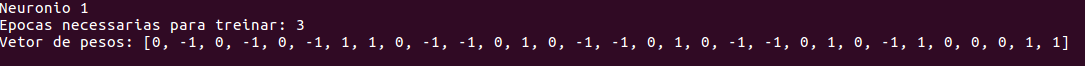
\includegraphics[scale=0.4]{Figures/E1PE1.png}
		\end{figure}
		
		\newpage
		
		\subsubsection{Saída para as representações distorcidas dos numerais 0 e 1 - com vetor de pesos inicialmente zerado}
		
		\begin{figure}[!h]
			\centering
			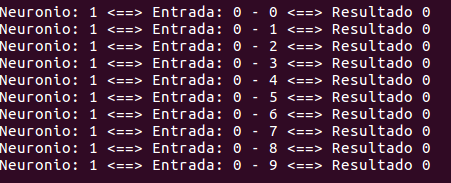
\includegraphics[scale=0.7]{Figures/E1S0.png}
		\end{figure}
		
		\begin{figure}[!h]
			\centering
			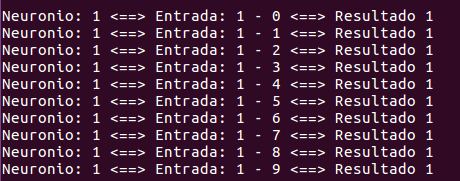
\includegraphics[scale=0.7]{Figures/E1S1.png}
		\end{figure}
		
		\subsubsection{Saída para as representações dos numerais 2, 3, 4, 5 - com vetor de pesos inicialmente zerado}
		
		\begin{figure}[!h]
			\centering
			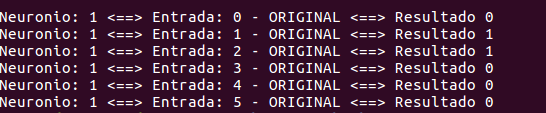
\includegraphics[scale=0.7]{Figures/E1SALL.png}
		\end{figure}
		
		\newpage
		
		\subsubsection{Vetor de pesos iniciamente aleatório}
		
		\begin{figure}[!h]
			\centering
			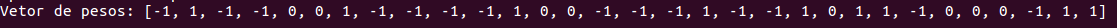
\includegraphics[scale=0.4]{Figures/E1P1R.png}
		\end{figure}
		
		\subsubsection{Número de épocas para se aprender um padrão e vetor de pesos final - com vetor de pesos inicialmente aleatório}
		
		\begin{figure}[!h]
			\centering
			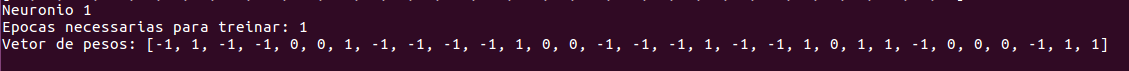
\includegraphics[scale=0.4]{Figures/E1PE1R.png}
		\end{figure}
		
		\newpage
		
		\subsubsection{Saída para as representações distorcidas dos numerais 0 e 1 - com vetor de pesos inicialmente aleatório}
		
		\begin{figure}[!h]
			\centering
			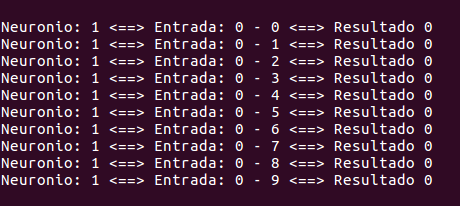
\includegraphics[scale=0.7]{Figures/E1S0R.png}
		\end{figure}
		
		\begin{figure}[!h]
			\centering
			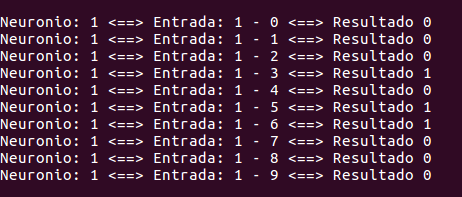
\includegraphics[scale=0.7]{Figures/E1S1R.png}
		\end{figure}
		
		\newpage
		
		\subsubsection{Saída para as representações dos numerais 2, 3, 4, 5 - com vetor de pesos inicialmente aleatório}
		
		\begin{figure}[!h]
			\centering
			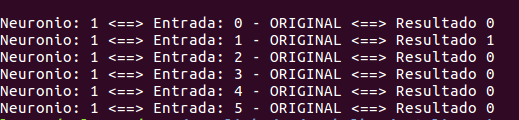
\includegraphics[scale=0.7]{Figures/E1SALLR.png}
		\end{figure}


	\subsection{Exercício 2}
		
		\subsubsection{Número de épocas para se aprender um padrão e vetor de pesos final - com vetor de pesos inicialmente zerado}
		
		\begin{figure}[!h]
			\centering
			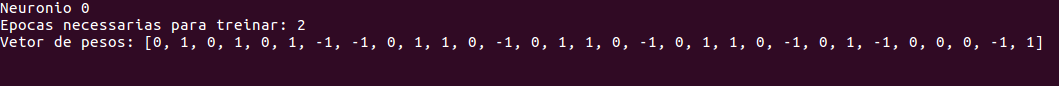
\includegraphics[scale=0.4]{Figures/E2PE0.png}
		\end{figure}
		
		\begin{figure}[!h]
			\centering
			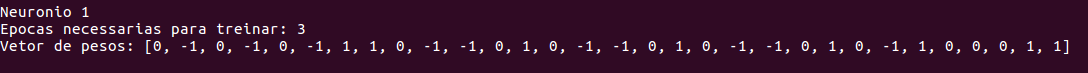
\includegraphics[scale=0.4]{Figures/E2PE1.png}
		\end{figure}
		
		\newpage
		
		\subsubsection{Saída para as representações distorcidas dos numerais 0 e 1 - com vetor de pesos inicialmente zerado}
		
		\begin{figure}[!h]
			\centering
			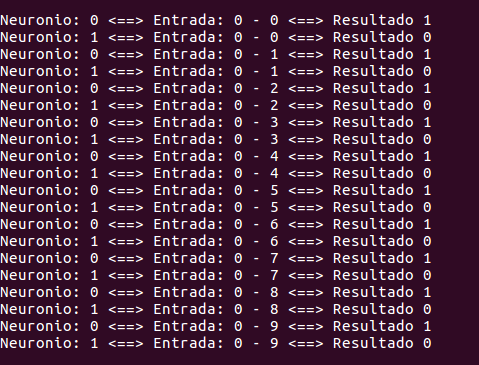
\includegraphics[scale=0.7]{Figures/E2S0.png}
		\end{figure}
		
		\begin{figure}[!h]
			\centering
			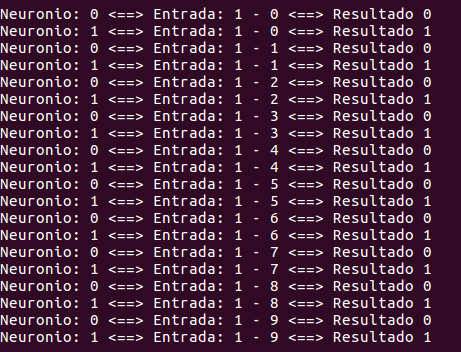
\includegraphics[scale=0.7]{Figures/E2S1.png}
		\end{figure}
		
		\newpage
		
		\subsubsection{Saída para as representações dos numerais 2, 3, 4, 5 - com vetor de pesos inicialmente zerado}
		
		\begin{figure}[!h]
			\centering
			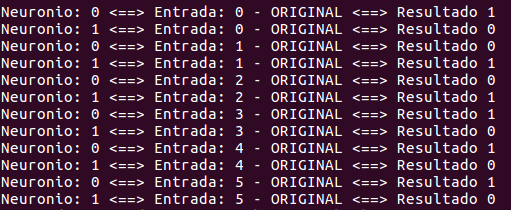
\includegraphics[scale=0.7]{Figures/E2SALL.png}
		\end{figure}
		
		\newpage
		\subsubsection{Vetor de pesos inicialmente aleatório}
			
		\begin{figure}[!h]
			\centering
			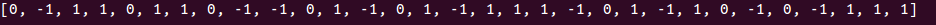
\includegraphics[scale=0.5]{Figures/E2PI0.png}
		\end{figure}
		
		\begin{figure}[!h]
			\centering
			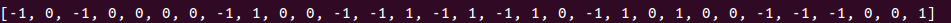
\includegraphics[scale=0.5]{Figures/E2PI1.png}
		\end{figure}

		\subsubsection{Número de épocas para se aprender um padrão e vetor de pesos final - com vetor de pesos inicialmente aleatório}
		
		\begin{figure}[!h]
			\centering
			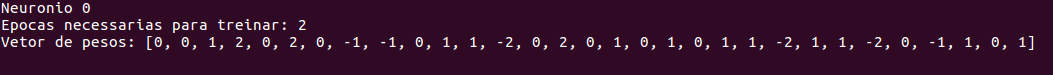
\includegraphics[scale=0.4]{Figures/E2PE0R.png}
		\end{figure}
		
		\begin{figure}[!h]
			\centering
			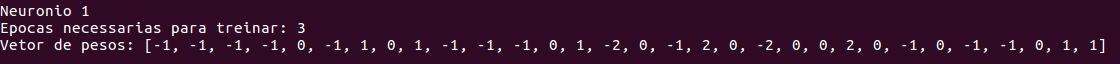
\includegraphics[scale=0.4]{Figures/E2PE1R.png}
		\end{figure}
		
		\newpage
		
		\subsubsection{Saída para as representações distorcidas dos numerais 0 e 1 - com vetor de pesos inicialmente aleatório}
		
		\begin{figure}[!h]
			\centering
			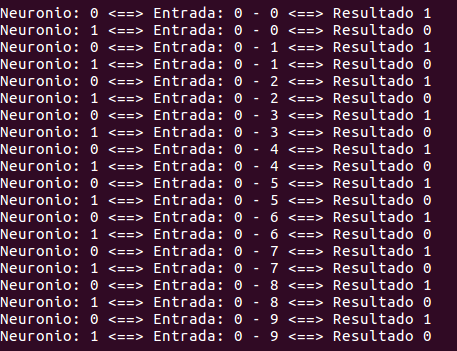
\includegraphics[scale=0.7]{Figures/E2S0R.png}
		\end{figure}
		
		\begin{figure}[!h]
			\centering
			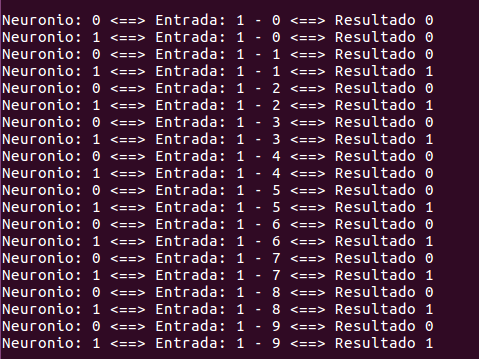
\includegraphics[scale=0.7]{Figures/E2S1R.png}
		\end{figure}
		
		\newpage
		
		\subsubsection{Saída para as representações distorcidas dos numerais 2, 3, 4, 5 - com vetor de pesos inicialmente aleatório}
		
		\begin{figure}[!h]
			\centering
			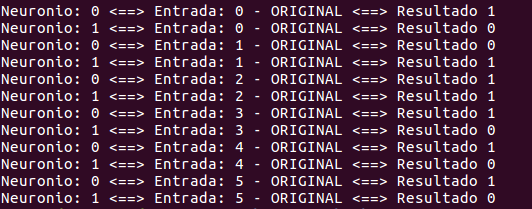
\includegraphics[scale=0.7]{Figures/E2SALLR.png}
		\end{figure}
		
	\subsection{Exercício 3}
		
		\subsubsection{Número de épocas para se aprender um padrão e vetor de pesos final - com vetor de pesos inicalmente zerado}
		
		\begin{figure}[!h]
			\centering
			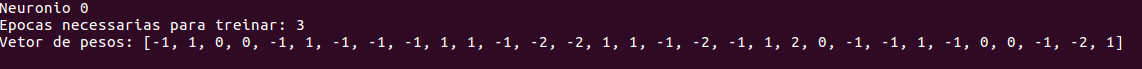
\includegraphics[scale=0.4]{Figures/E3PE0.png}
		\end{figure}
		
		\begin{figure}[!h]
			\centering
			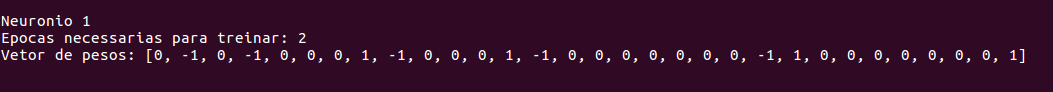
\includegraphics[scale=0.4]{Figures/E3PE1.png}
		\end{figure}
		
		\begin{figure}[!h]
			\centering
			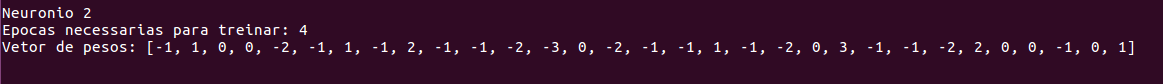
\includegraphics[scale=0.4]{Figures/E3PE2.png}
		\end{figure}
		
		\begin{figure}[!h]
			\centering
			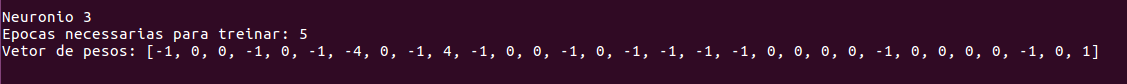
\includegraphics[scale=0.4]{Figures/E3PE3.png}
		\end{figure}
		
		\begin{figure}[!h]
			\centering
			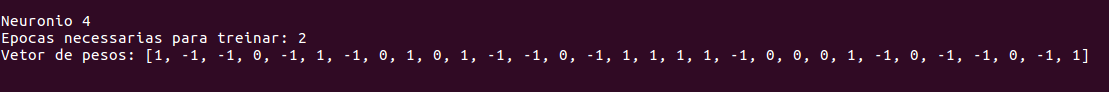
\includegraphics[scale=0.4]{Figures/E3PE4.png}
		\end{figure}
		
		\begin{figure}[!h]
			\centering
			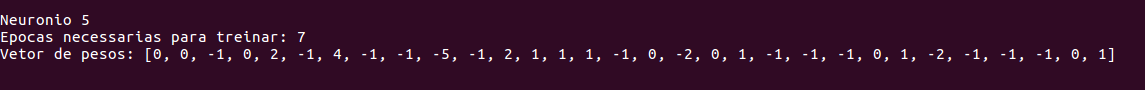
\includegraphics[scale=0.4]{Figures/E3PE5.png}
		\end{figure}
			
		\newpage
		
		\subsubsection{Saída para as representações distorcidas dos numerais 0, 1, 2, 3, 4, 5 - com vetor de pesos inicalmente zerado}
		
		\begin{figure}[!h]
			\centering
			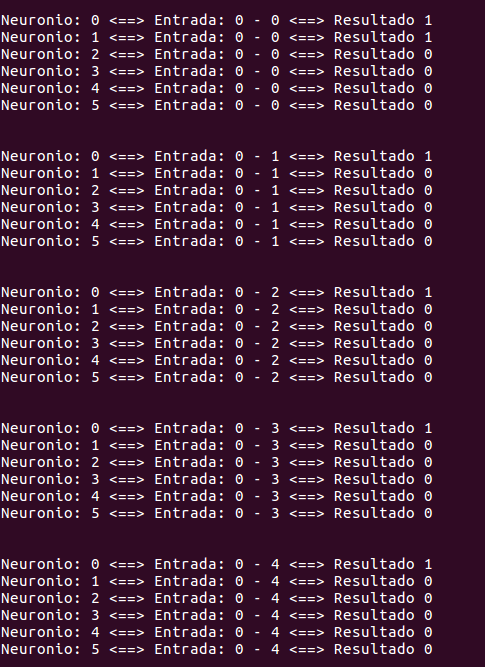
\includegraphics[scale=0.5]{Figures/E3S0P1.png}
		\end{figure}
		
		\begin{figure}[!h]
			\centering
			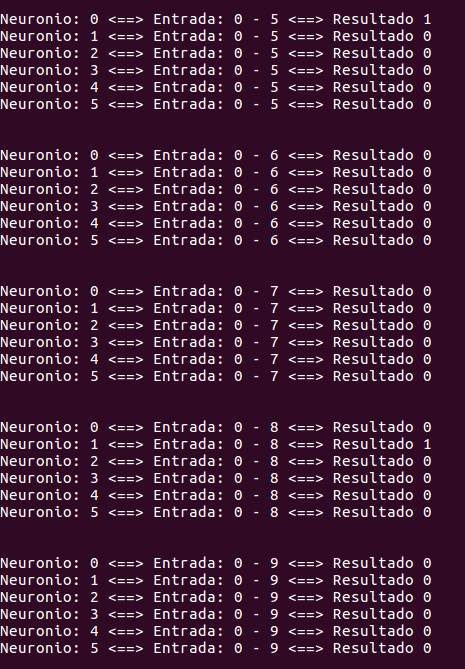
\includegraphics[scale=0.5]{Figures/E3S0P2.png}
		\end{figure}
		
		\begin{figure}[!h]
			\centering
			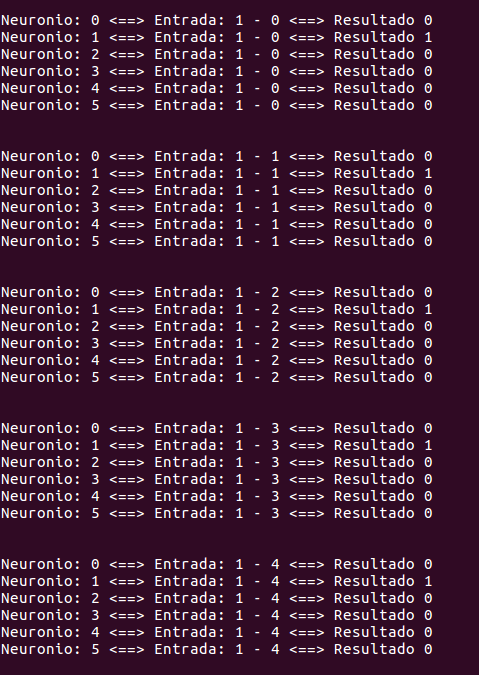
\includegraphics[scale=0.5]{Figures/E3S1P1.png}
		\end{figure}
		
		\begin{figure}[!h]
			\centering
			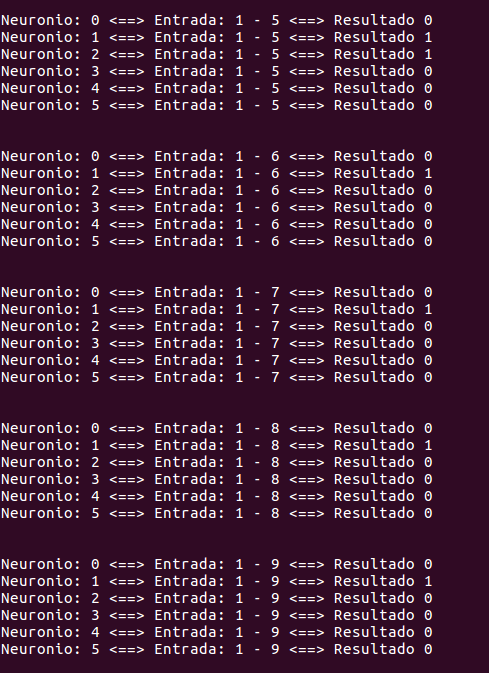
\includegraphics[scale=0.5]{Figures/E3S1P2.png}
		\end{figure}
		
		\begin{figure}[!h]
			\centering
			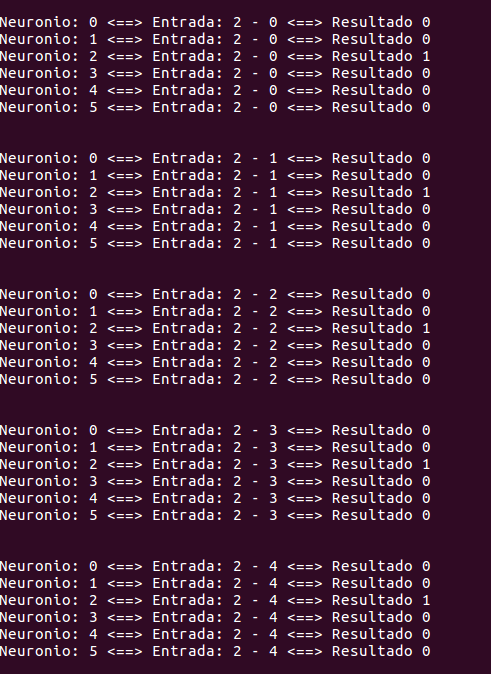
\includegraphics[scale=0.5]{Figures/E3S2P1.png}
		\end{figure}
		
		\begin{figure}[!h]
			\centering
			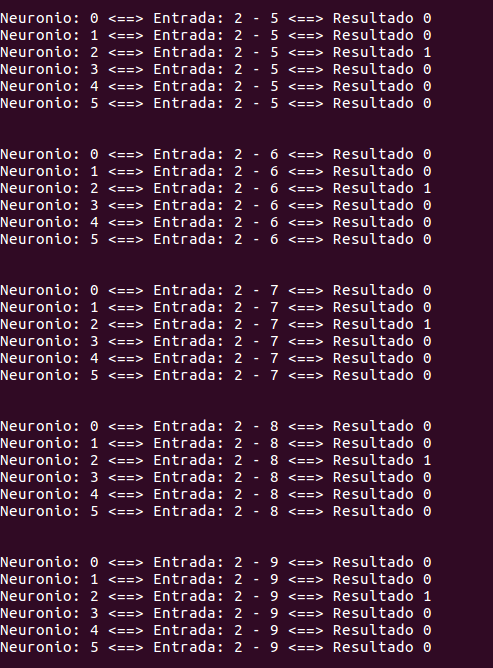
\includegraphics[scale=0.5]{Figures/E3S2P2.png}
		\end{figure}
		
		\begin{figure}[!h]
			\centering
			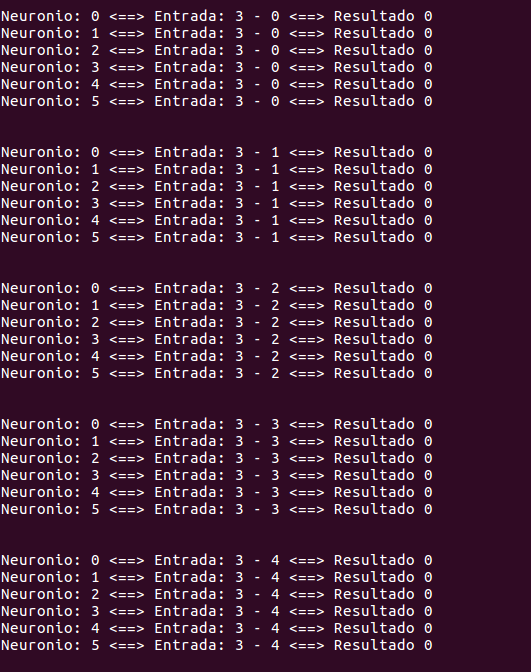
\includegraphics[scale=0.5]{Figures/E3S3P1.png}
		\end{figure}
		
		\begin{figure}[!h]
			\centering
			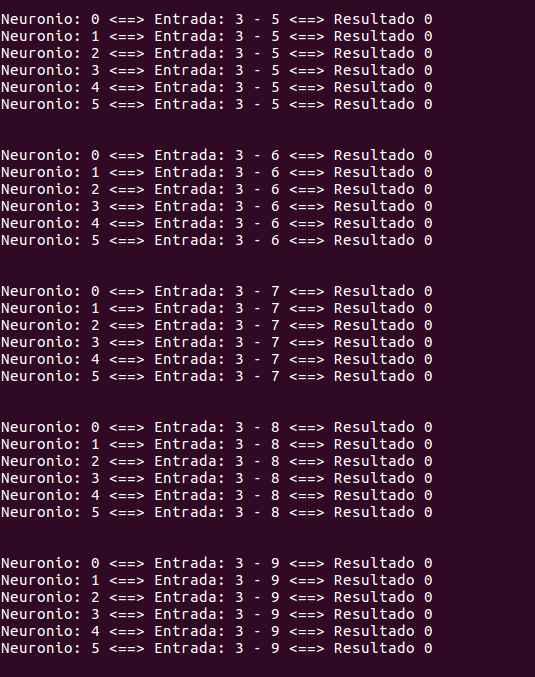
\includegraphics[scale=0.5]{Figures/E3S3P2.png}
		\end{figure}
		
		\begin{figure}[!h]
			\centering
			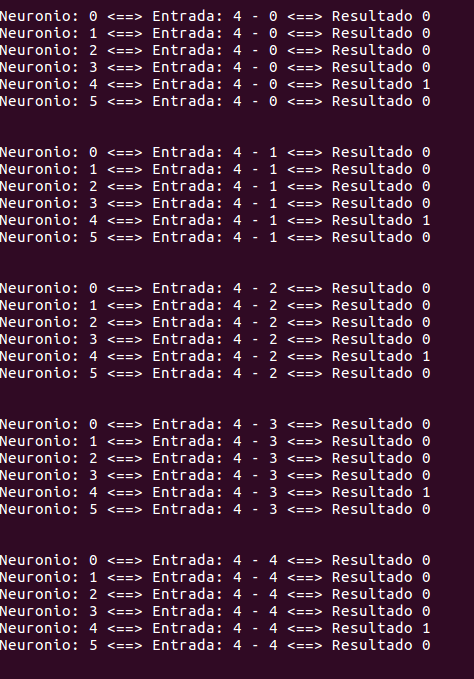
\includegraphics[scale=0.5]{Figures/E3S4P1.png}
		\end{figure}
		
		\begin{figure}[!h]
			\centering
			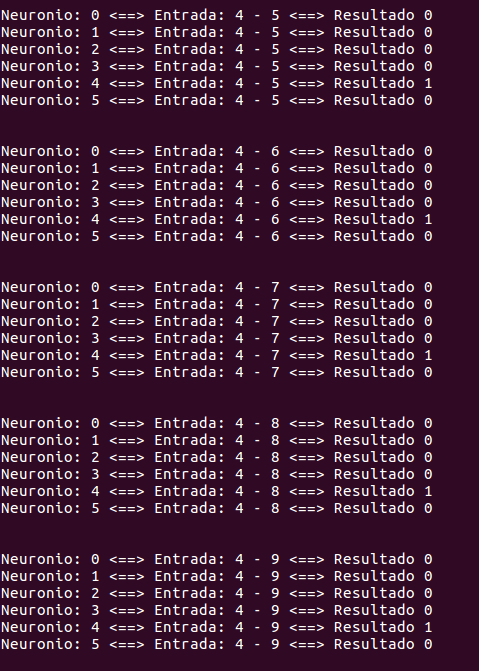
\includegraphics[scale=0.5]{Figures/E3S4P2.png}
		\end{figure}
		
		\begin{figure}[!h]
			\centering
			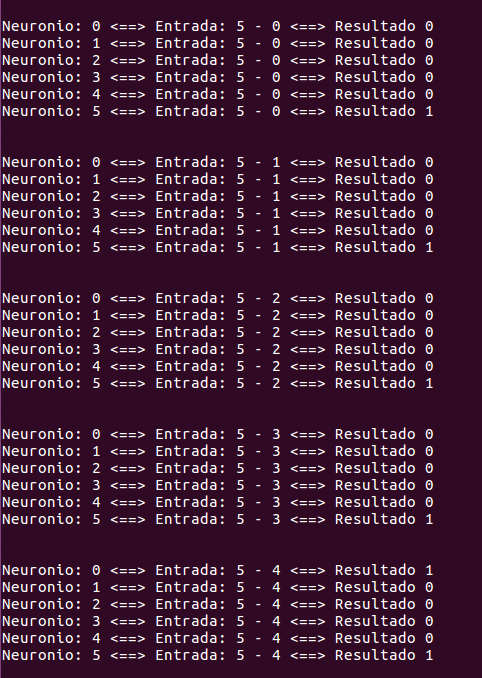
\includegraphics[scale=0.5]{Figures/E3S5P1.png}
		\end{figure}
		
		\begin{figure}[!h]
			\centering
			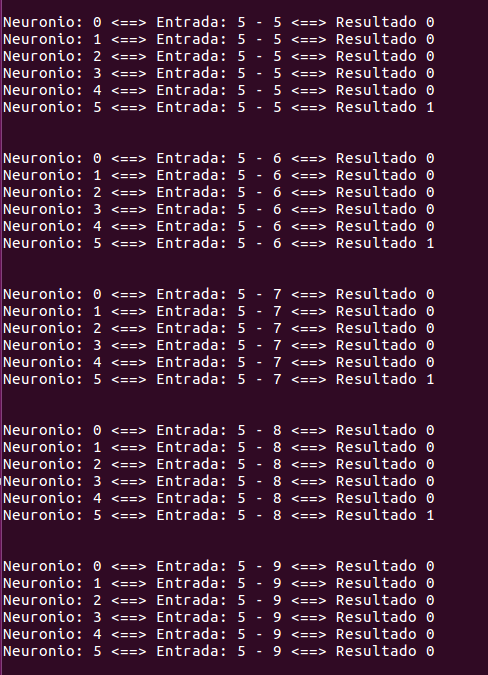
\includegraphics[scale=0.5]{Figures/E3S5P2.png}
		\end{figure}
		
		\newpage
		
		\subsubsection{Saída para as representações das letras A, C, E, H, N, T - com vetor de pesos inicalmente zerado}
		
		\begin{figure}[!h]
			\centering
			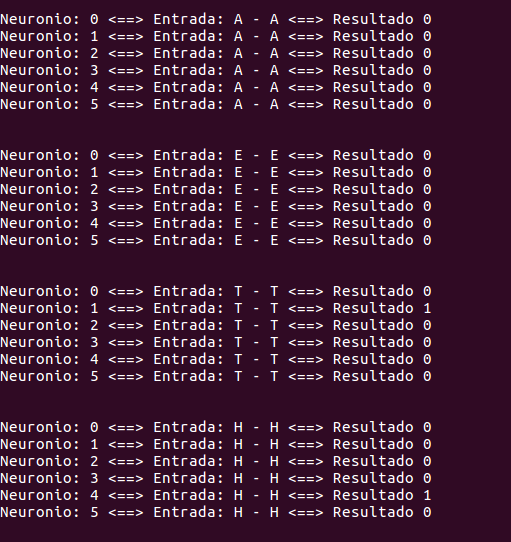
\includegraphics[scale=0.5]{Figures/E3SLP1.png}
		\end{figure}
		
		\begin{figure}[!h]
			\centering
			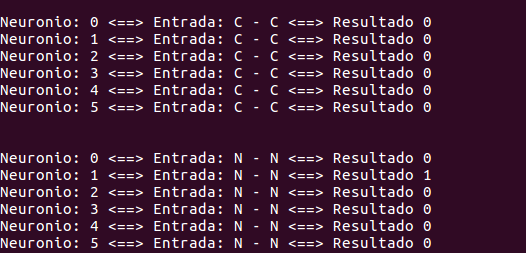
\includegraphics[scale=0.5]{Figures/E3SLP2.png}
		\end{figure}
		
		\newpage
		
		\subsubsection{Vetor de pesos inicalmente aleatório}
		
		\begin{figure}[!h]
		    \centering
		    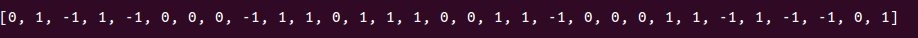
\includegraphics[scale=0.4]{Figures/E3PI0.png}
		\end{figure}
		
		\begin{figure}[!h]
			\centering
			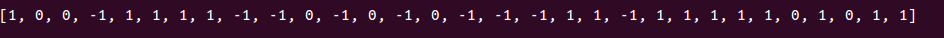
\includegraphics[scale=0.4]{Figures/E3PI1.png}
		\end{figure}
		
		\begin{figure}[!h]
			\centering
			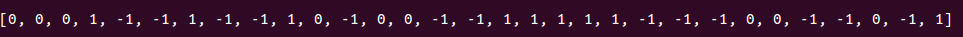
\includegraphics[scale=0.4]{Figures/E3PI2.png}
		\end{figure}
		
		\begin{figure}[!h]
			\centering
			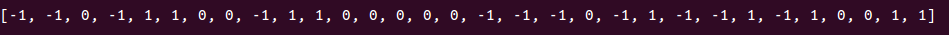
\includegraphics[scale=0.4]{Figures/E3PI3.png}
		\end{figure}
		
		\begin{figure}[!h]
			\centering
			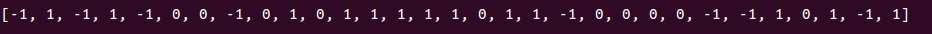
\includegraphics[scale=0.4]{Figures/E3PI4.png}
		\end{figure}
		
		\begin{figure}[!h]
			\centering
			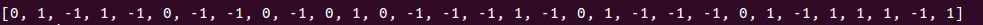
\includegraphics[scale=0.4]{Figures/E3PI5.png}
		\end{figure}
			
		\newpage
		
		\subsubsection{Número de épocas para se aprender um padrão e vetor de pesos final - com vetor de pesos inicalmente aleatório}
		
		\begin{figure}[!h]
			\centering
			\includegraphics[scale=0.4]{Figures/E3PE0R.png}
		\end{figure}
		
		\begin{figure}[!h]
			\centering
			\includegraphics[scale=0.4]{Figures/E3PE1R.png}
		\end{figure}
		
		\begin{figure}[!h]
			\centering
			\includegraphics[scale=0.4]{Figures/E3PE2R.png}
		\end{figure}
		
		\begin{figure}[!h]
			\centering
			\includegraphics[scale=0.4]{Figures/E3PE3R.png}
		\end{figure}
		
		\begin{figure}[!h]
			\centering
			\includegraphics[scale=0.4]{Figures/E3PE4R.png}
		\end{figure}
		
		\begin{figure}[!h]
			\centering
			\includegraphics[scale=0.4]{Figures/E3PE5R.png}
		\end{figure}
		
		\newpage
		
		\subsubsection{Saída para as representações distorcidas dos numerais 0, 1, 2, 3, 4, 5 - com vetor de pesos inicalmente aleatório}
		
		\begin{figure}[!h]
			\centering
			\includegraphics[scale=0.5]{Figures/E3S0P1R.png}
		\end{figure}
		
		\begin{figure}[!h]
			\centering
			\includegraphics[scale=0.5]{Figures/E3S0P2R.png}
		\end{figure}
		
		\begin{figure}[!h]
			\centering
			\includegraphics[scale=0.5]{Figures/E3S1P1R.png}
		\end{figure}
		
		\begin{figure}[!h]
			\centering
			\includegraphics[scale=0.5]{Figures/E3S1P2R.png}
		\end{figure}
		
		\begin{figure}[!h]
			\centering
			\includegraphics[scale=0.5]{Figures/E3S2P1R.png}
		\end{figure}
		
		\begin{figure}[!h]
			\centering
			\includegraphics[scale=0.5]{Figures/E3S2P2R.png}
		\end{figure}
		
		\begin{figure}[!h]
			\centering
			\includegraphics[scale=0.5]{Figures/E3S3P1R.png}
		\end{figure}
		
		\begin{figure}[!h]
			\centering
			\includegraphics[scale=0.5]{Figures/E3S3P2R.png}
		\end{figure}
		
		\begin{figure}[!h]
			\centering
			\includegraphics[scale=0.5]{Figures/E3S4P1R.png}
		\end{figure}
		
		\begin{figure}[!h]
			\centering
			\includegraphics[scale=0.5]{Figures/E3S4P2R.png}
		\end{figure}
		
		\begin{figure}[!h]
			\centering
			\includegraphics[scale=0.5]{Figures/E3S5P1R.png}
		\end{figure}
		
		\begin{figure}[!h]
			\centering
			\includegraphics[scale=0.5]{Figures/E3S5P2R.png}
		\end{figure}
		
		\newpage
		
		\subsubsection{Saída para as representações das letras A, C, E, H, N, T - com vetor de pesos inicalmente aleatório}
		
		\begin{figure}[!h]
			\centering
			\includegraphics[scale=0.5]{Figures/E3SLP1R.png}
		\end{figure}
		
		\begin{figure}[!h]
			\centering
			\includegraphics[scale=0.5]{Figures/E3SLP2R.png}
		\end{figure}
		
	
\end{document}
